\documentclass[12pt,letter]{article}
\usepackage{mathptmx} % added for time new roman font
\usepackage[left=1in,right=1in,top=1in,bottom=1in]{geometry}
\usepackage[latin1]{inputenc}
\usepackage{amsmath}

% defines all example enviorment
\usepackage[framemethod=tikz]{mdframed} % added for the box around examples
\newtheorem{ex}{Example}
\numberwithin{ex}{section} % allows for the use of example numbers that lign up with the section numbers
\newenvironment{example}{\begin{mdframed}[middlelinewidth=0.5mm]\begin{ex}\normalfont}{\end{ex}\end{mdframed}}

% defines all review enviorment
\usepackage[framemethod=tikz]{mdframed} % added for the box around examples
\newtheorem{re}{Review}
\numberwithin{re}{section} % allows for the use of example numbers that lign up with the section numbers
\newenvironment{review}{\begin{mdframed}[middlelinewidth=2mm,roundcorner=20pt]\begin{re}\normalfont}{\end{re}\end{mdframed}}

% defines the quotation enviorment 
\usepackage{xcolor}
\newcommand{\quotebox}[2]{\begin{center}\fcolorbox{white}{blue!15!gray!15}{\begin{minipage}{0.9\linewidth}\vspace{10pt}\center\begin{minipage}{0.8\linewidth}{\space\Huge``}{#1}{\Huge''}{\break\null\hfill} {\small #2}  \end{minipage}\medbreak\end{minipage}}\end{center}}

% defines the definition enviorment 
\newcommand{\definitionbox}[2]{\begin{center}\fcolorbox{white}{blue!15!gray!15}{\begin{minipage}{0.9\linewidth}\vspace{10pt}\center\begin{minipage}{0.8\linewidth} {{\textbf{Definition} - }{#1}: {#2}}\end{minipage}\medbreak\end{minipage}}\end{center}}

\usepackage{amsfonts}
\usepackage{amssymb}
\usepackage{graphicx}
\usepackage{float}
\usepackage{booktabs}
%\usepackage{parskip} % remove all the paragraph indents
\usepackage[textsize=tiny]{todonotes}


\usepackage{setspace}
\usepackage[colorlinks=true]{hyperref}
\usepackage{textcomp} 
\usepackage{multicol} 

% added for MATLAB code
\usepackage[framed]{matlab-prettifier}
\let\ph\mlplaceholder % shorter macro
\lstMakeShortInline"

\lstset{
  style              = Matlab-editor,
  basicstyle         = \mlttfamily,
  escapechar         = ",
  mlshowsectionrules = true,
}



\usepackage{color} % color added for editing
\newcommand{\bl}[1]{\textcolor[rgb]{0.00,0.00,1.00}{#1}}
\newcommand{\gr}[1]{\textcolor[rgb]{0.00,0.50,0.00}{#1}}
\newcommand{\rd}[1]{\textcolor[rgb]{0.75,0.00,0.00}{#1}}
\newcommand{\tl}[1]{\textcolor[rgb]{0,0.6,0.60}{#1}}



%%%%%%%		define the symbols for positive directions		%%%%%%
\makeatletter													%%	
																%%					
\newcommand*\curveplus{% positive counterclockwise				%%
  \mathbin{\rotatebox[origin=c]{90}{$\m@th\curvearrowleft$}+}}	%%
																%%
\newcommand*\rightplus{% positive right							%%
  \mathpalette\@rightplus\relax}								%%
\newcommand*\@rightplus[1]{%									%%
  \mathbin{\vcenter{\hbox{$\m@th\overset{#1+}{\to}$}}}}			%%
																%%	
\newcommand*\upplus{% positive up								%%
  \mathbin{+\mathord\uparrow}}									%%
																%%			
\newcommand*\downplus{% positive down							%%		
  \mathbin{+\mathord\downarrow}}								%%
  																%%		
\newcommand*\downrightplus{% positive down and right			%%	
  \mathbin{+ \rotatebox[origin=c]{-30}{$\m@th\rightarrow$}}}	%%
\makeatother 													%%	
%%%%%%%%%%%%%%%%%%%%%%%%%%%%%%%%%%%%%%%%%%%%%%%%%%%%%%%%%%%%%%%%%%


\usepackage{mathtools}          %loads amsmath as well added for the piece wise function
\DeclarePairedDelimiter\Floor\lfloor\rfloor
\DeclarePairedDelimiter\Ceil\lceil\rceil

 
\newcounter{NumberInTable}
\newcommand{\LTNUM}{\stepcounter{NumberInTable}{(\theNumberInTable)}}

\newcommand{\Laplace}[1]{\ensuremath{\mathcal{L}{\left[#1\right]}}}
\newcommand{\InvLap}[1]{\ensuremath{\mathcal{L}^{-1}{\left[#1\right]}}}
\renewcommand{\textuparrow}{$\uparrow$}


\begin{document}
	
	% set the section number, along with figure and equation numbers
	\setcounter{section}{6}	
	\setcounter{figure}{0}   
	\renewcommand\thefigure{\thesection.\arabic{figure}}
	\setcounter{equation}{0}   
	\renewcommand\theequation{\thesection.\arabic{equation}}	
	
	\section{Structural Dynamics}	
	
	\subsection{Single-story frame}


The dynamic response of civil infrastructures, including buildings, bridges, and towers, can be studied by applying fundamental vibrations concepts studied in the previous chapters. 

Let's start by considering the single-story frame shown in Fig. \ref{fig:one_story_frame_example} (a) in free vibration (no external load is applied to the structure). The frame has height $H$ and bay width $L$. As shown in Fig. \ref{fig:one_story_frame_example}, the frame consists of two columns with modulus of elasticity $E$ and moment of inertia (second moment of the cross sectional area) $I$. The columns are fixed at the base. The frame in Fig. \ref{fig:one_story_frame_example} (a) can be modeled as a single-degree of freedom (SDOF) system under the following assumptions:

\begin{itemize}
	\item Shear building: flexible columns ($EI \neq 0$), beam infinitely rigid ($EI_b$ = $\infty$), axial deformations of beams and columns negligible ($EA$ = 0);
	\item Lumped mass system: floor-mass concentrated at the floor level.
\end{itemize}

Fig. \ref{fig:single_} (b) illustrates a SDOF with mass $m$ and stiffness $k$ that can be used to model the dynamic behavior of the single-story frame considering no damping ($\zeta$ = 0). 

\begin{figure}[H]
	\centering
	\includegraphics{../figures/Single_story_frame.png}
	\caption{(a) Single story frame; (b) undamped single degree of freedom system.}
	\label{fig:one_story_frame_example}
\end{figure}

%\begin{figure}[H]
%	\centering
%	\includegraphics[]{Figures_LM/Single_story_frame.png}
%	\caption{(a) Single story frame; (b) undamped single degree of freedom system.}
%	\label{fig:single_a}
%\end{figure}
%
%\begin{figure}[H]
%    \centering
%    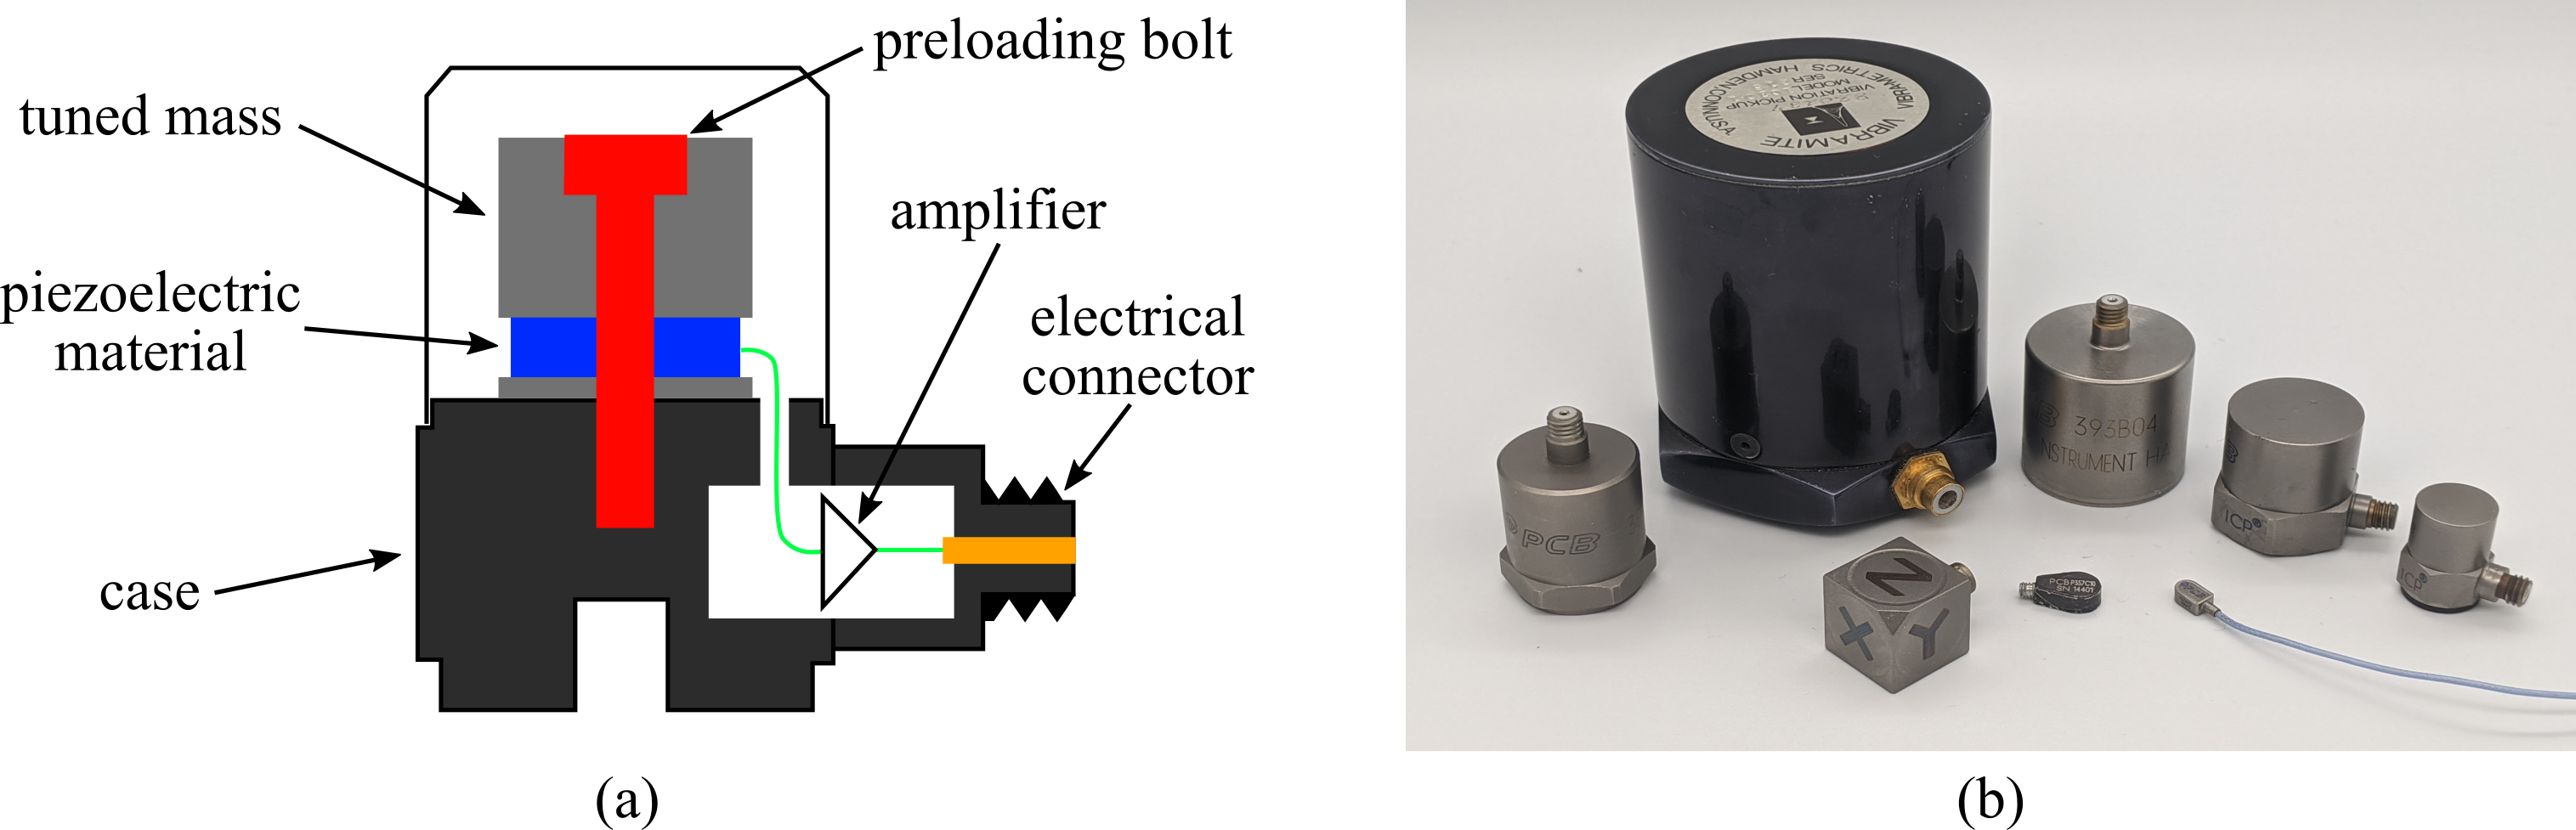
\includegraphics[]{../Figures/accelerometers.png}
%    \caption{Integrated Electronics Piezo-Electric (IEPE) accelerometers, showing: (a) the cross section of a typical IEPE) accelerometer with key components annotated, and; (b) selection of IEPE accelerometers for various applications.}
%    \label{fig:accelerometersss}
%\end{figure} 



\pagebreak
The response of a SDOF system can be written in general notation as:

\begin{equation}
x(t) = x_0\text{cos}(\omega_n t) + \frac{v_0}{\omega_n}\text{sin}(\omega_n t)
\end{equation}

where $\omega_n$ is the natural frequency of the frame, $x_0$ and $v_0$ are the initial conditions. In order to find $\omega_n$, we need to calculate the stiffness of the system. The mass is usually given. 

The stiffness of the system can be found by applying the Hooke's law: $F = k x$. To find $k$, let's imagine to apply an arbitrary lateral force $F$ to the frame and analyze a single column. At the top, the column will be subjected to a force $F$ and to a moment $M_0$, as schematically shown in Fig. \ref{fig:columns_draw} (a). Applying the equilibrium equations to the column, it can be found that $M_0 = \frac{F H}{2}$. 

\begin{figure}[H]
	\centering
	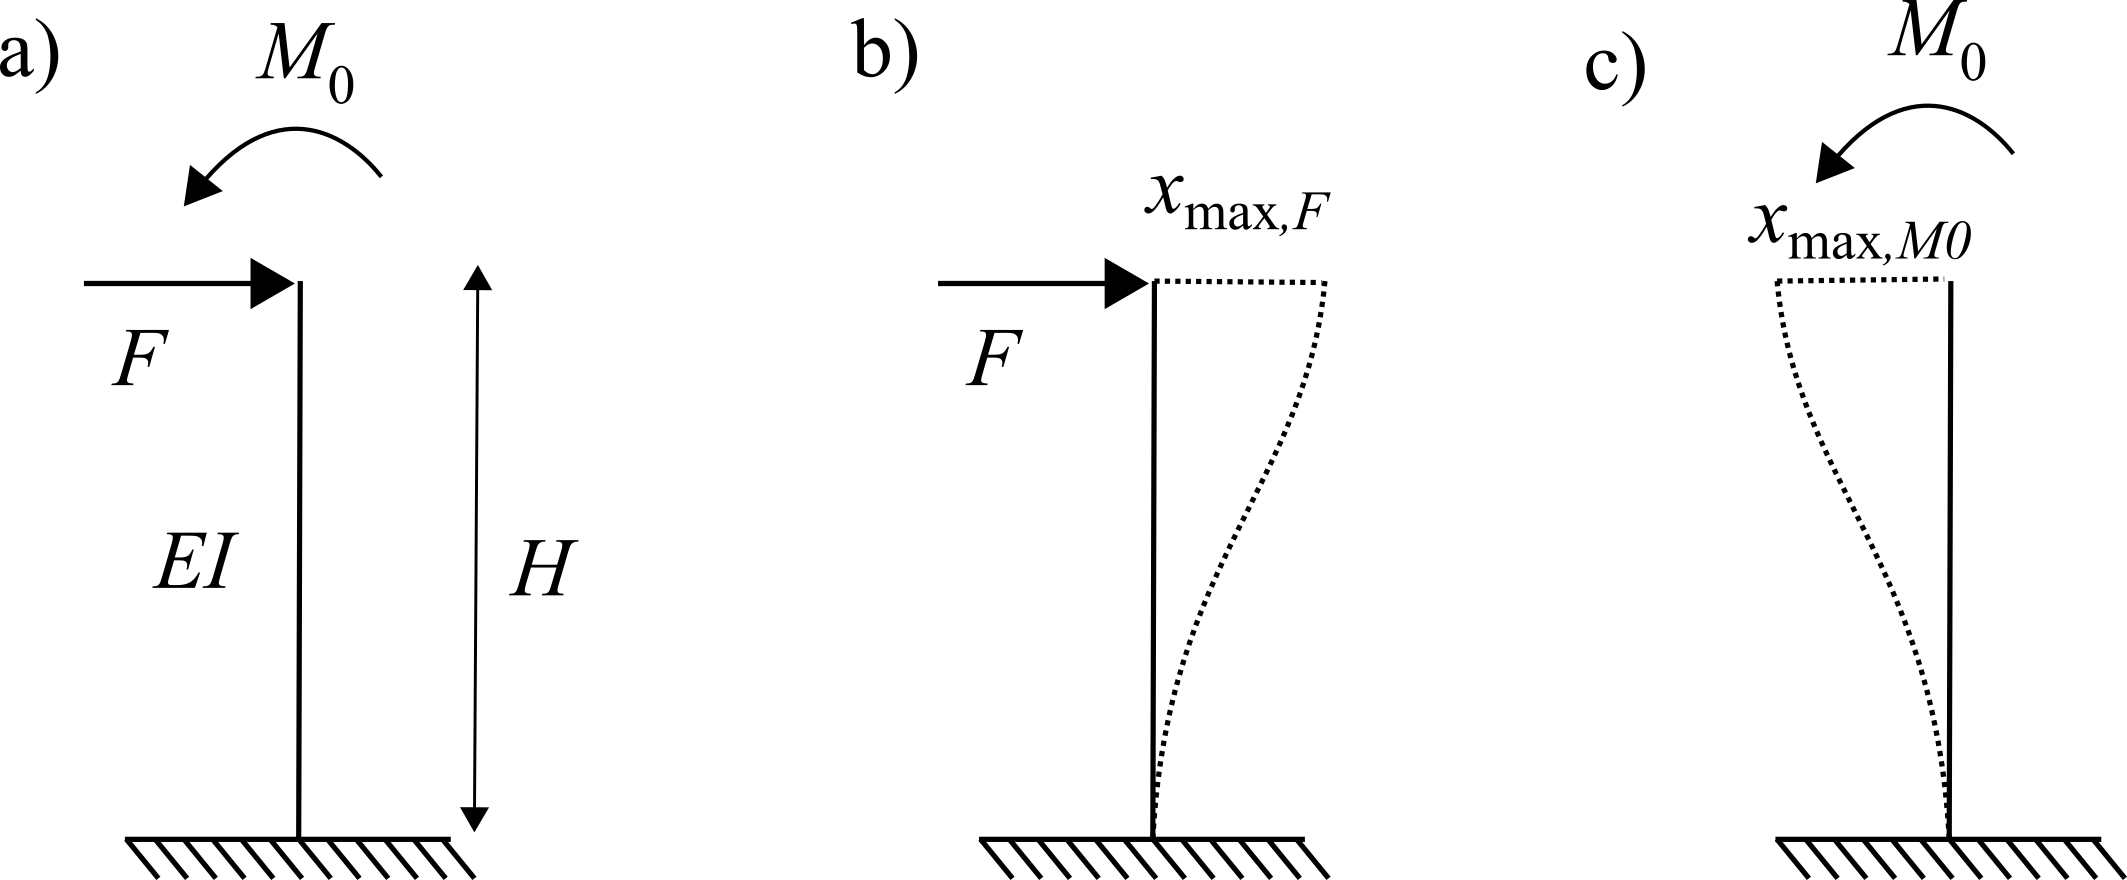
\includegraphics{../figures/frame_columns.png}
	\caption{Single column subjected to: (a) force and moment; (b) force only; (c) moment only.}
	\label{fig:columns_draw}
\end{figure}


Since the system is linear, we can calculate the effects of $F$ and $M_0$ separately and then summed them together (superposition principle). The maximum deflection due to $F$ occurs at the top of the column, as shown in Fig. \ref{fig:columns_draw} (b), and it is equal to:

\begin{equation} \label{Eq_xmax_F}
x_{\text{max},F} = \frac{FH^3}{3EI}
\end{equation}

while the maximum deflection caused by $M_0$ (Fig. \ref{fig:columns_draw} (c)) is:

\begin{equation} \label{Eq_xmax_M0}
x_{\text{max},M0} = \frac{M_0H^2}{2EI}
\end{equation}

The displacements in Eq. (\ref{Eq_xmax_F}) and (\ref{Eq_xmax_M0}) were found using engineering tables. The total displacement $x$ at the top of the column is obtained from the sum of the two displacements:

\begin{equation} \label{Eq_xmax_tot}
x =  \frac{FH^3}{3EI} - \frac{M_0H^2}{2EI}
\end{equation}

where the $x_{\text{max},M0}$ is negative in sign because the displacement caused by $M_0$ goes in opposite direction to $x_{\text{max},F}$. Replacing $M_0 = \frac{F H}{2}$ in Eq. (\ref{Eq_xmax_tot}):

\begin{equation}
x = \frac{FH^3}{3EI} - \frac{FH^3}{4EI} = \frac{FH^3}{12EI}
\end{equation}


Applying Hooke's law:
\begin{equation}
F = k_c x = k_c \frac{FH^3}{12EI}
\end{equation}

where $k_c$ is the stiffness of the column. Therefore:

\begin{equation}
k_c = \frac{12EI}{H^3}
\end{equation}

Since the frame has two columns, the total stiffness of the SDOF system will be:

\begin{equation}
k = \sum_{columns}^{} k_c = \sum_{2}^{} \frac{12EI} {H^3}
\end{equation}

where $k$ is also called \emph{lateral stiffness}. Note that the lateral stiffness of the frame is independent on the length of the bay $L$ and it depends only on the properties of the columns ($E$, $I$, and $H$). It is possible at this point to calculate the natural frequency of the frame:

\begin{equation} \label{omega_frame}
\omega_n = \sqrt{\frac{k}{m}} = \sqrt{\frac{\sum_{2}^{} \frac{12EI} {H^3}}{m}}
\end{equation}

If the columns have same properties, Eq. (\ref{omega_frame}) becomes:

\begin{equation}
\omega_n = \sqrt{\frac{k}{m}} = \sqrt{\frac{24EI}{H^3m}}
\end{equation}


Finally, the response of the system to initial conditions $x_0$ and ${v_0}$ can be obtained:

\begin{equation}
x(t) = x_0\text{cos}(\omega_n t) + \frac{v_0}{\omega_n}\text{sin}(\omega_n t)
\end{equation}	

\pagebreak


\begin{example}
	
Let's consider the single-story frame shown in Fig. \ref{fig:one_story_frame_example} with mass $m$ = 0.15 kip $s^2$/ft, $L$ = 12 ft, $EI$= 1800 kip $ft^2$. a) Determine the EOM and the natural period of the frame; b) assume that the moment of inertia of the right column is $2I$. Will the EOM change?

\vspace{1ex}

\noindent$Solution$:

\vspace{1ex}

a) The frame can be modeled as a single-degree of freedom in free vibration. Therefore, the EOM is:

\begin{equation}
	m \ddot{x} + k x = 0
\end{equation}

The lateral stiffness of the system is:

\begin{equation}
k = \sum_{columns}^{} k_c = \sum_{2}^{} \frac{12EI} {H^3} = \frac{24 EI}{H^3}
\end{equation}

Thus, the natural frequency and period are:

\begin{equation}
\omega_n = \sqrt{\frac{k}{m}} = \sqrt{\frac{24 EI}{m H^3}} = \sqrt{\frac{1800}{0.15 \cdot 12^3}} = 12.91 \frac{rad}{s}
\end{equation}

\begin{equation}
T_n =\frac{2 \pi}{\omega_n} = 0.48 s
\end{equation}

b) The EOM won't change, but the lateral stiffness of the system will be: 

\begin{equation}
k = \sum_{columns}^{} k_c = \frac{12EI} {H^3} + \frac{24EI} {H^3} = \frac{36 EI}{H^3}
\end{equation}

	
\end{example}



The same principle can be applied to a single-story frame with damping ratio $\zeta \neq$ 0. In this case, the displacement of the frame will be given by:

\begin{equation}
x(t) = e^{(-\zeta\omega_nt)} \left( \frac{({v_0} + x_0)\omega_n}{\omega_d} \text{cos}(\omega_d t) + x_0 \text{sin}(\omega_dt) \right)
\end{equation} 

where $\omega_d$ is the damped natural frequency of the system:

\begin{equation}
\omega_d = \omega_n \sqrt{1 - \zeta^2}
\end{equation}



\subsection{Duhamel's Integral}

In Chapter 4, the frequency response method was used to solve the EOM of a SDOF system subjected to an arbitrary force. Here, an alternative method widely employed in structural dynamics to find the solution of the EOM is presented. This method exploits a specif integral, named Duhamel's integral. 

Let's consider an underdamped SDOF system subjected to an arbitrary force $F$($t$). The EOM is:


\begin{equation}
m \ddot{x} + c \dot{x} + k x = F(t)
\end{equation}

Let's assume that the system is at rest: $x$(0) = 0 and $\dot{x}$ = 0. The assumption underlying the Duhamel's integral method is that a generic force $F$($t$) can be expressed as a sequence of impulses of very small duration and the response of the system as the sum of the response to individual unit impulses. 

An impulsive force can be defined as a very large force applied in a very short time interval. Fig. \ref{fig:impulsive_force} (a) shows an impulsive force $F(t) = \frac{1}{\epsilon}$ applied at time $t = \tau$. Assuming to apply an impulsive force to a generic mass $m$ and applying Netwon's second law:

\begin{equation}
m \ddot{x} = F(t)
\end{equation}

and integrating both sides between two generic time instants $t_1$ and $t_2$ yields:

\begin{equation}
\int_{t_1}^{t_2} F(t) dt = m (\dot{x}_1 - \dot{x}_2)
\end{equation}

where the left-hand side of the equation represents the magnitude of the force and the right-hand side the change in momentum. 

In the limit case in which $\epsilon$ tends to 0, $F(t)$ tends to 1 and the impulsive force is called \emph{unit impulse}. In the case of a unit impulse, $\int_{t_1}^{t_2} F(t) dt = 1$ and $t_1$ tends to $t_2$. Therefore, the velocity of the mass can be found as:

\begin{equation} \label{Eq_vel}
\dot{x}(\tau)=\frac{1}{m}
\end{equation}

A similar concept applies to a SDOF system. Since the impulse is applied in a very short time interval, the spring and the damper do not have the time to react. When we apply a unit impulse to an underdamped SDOF, the system will start vibrating with velocity $\dot{x}(\tau)$ given by Eq. (\ref{Eq_vel}) and displacement $x(\tau) = 0$. The response of the system is given by the following equation:


\begin{equation}
x(t) = h(t - \tau) = \frac{1}{m \omega_d} e^{-\zeta \omega_n (t - \tau)} sin(\omega_d (t - \tau))
\end{equation}

where $\tau$ is the time instant at which the impulse is applied. Note that the Dirac delta function $\delta(t - \tau)$ mathematically defines a unit impulse centered at $t = \tau$.

\vspace{2ex}


\begin{figure}[H]
	\centering
	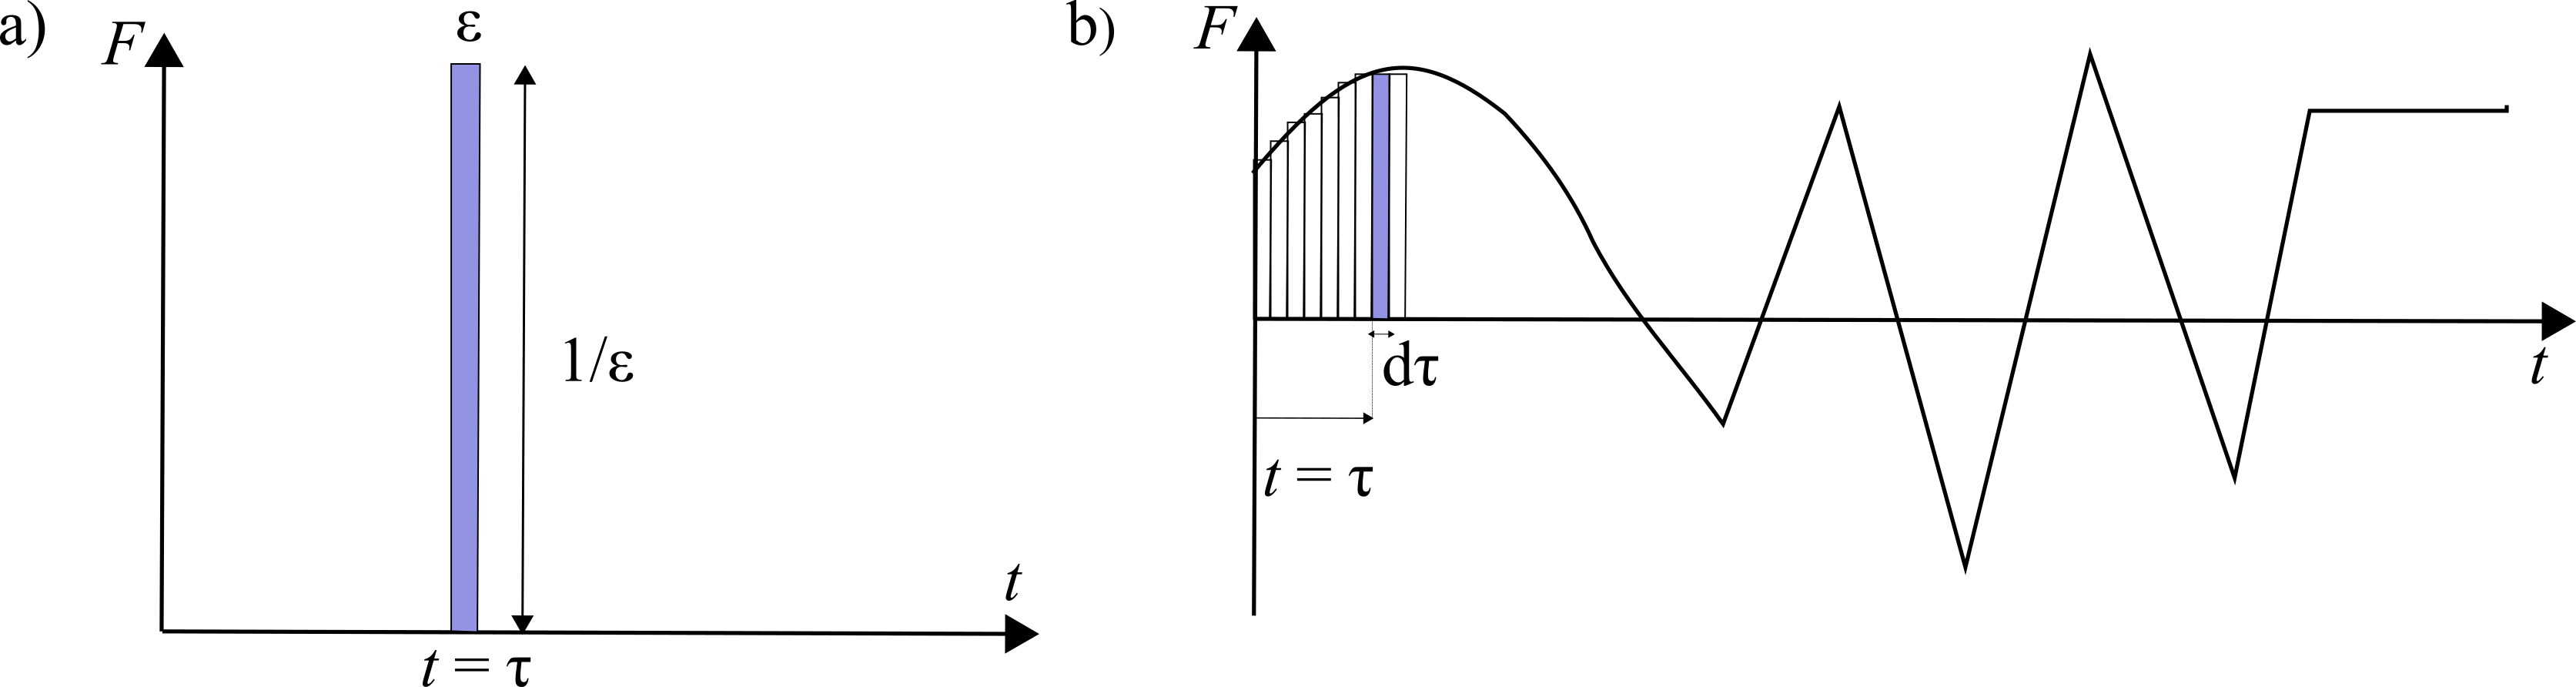
\includegraphics{../figures/Structural_Impulse.png}
	\caption{(a) Impulsive force; (b) arbitrary force decomposed in a series of impulses.}
	\label{fig:impulsive_force}
\end{figure}

Let's now consider a force $F(t)$ varying arbitrarily with time. As shown in Fig. \ref{fig:impulsive_force} (b), $F(t)$ can be represented as a sequence of infinitesimaly short impulses. The response of a linear system to $F(t)$ can be therefore expressed as the response to a series impulses, following:

\begin{equation} \label{Eq_impulses}
x(t) = \int_{0}^{t} p(\tau) h(t - \tau) d\tau
\end{equation}

where $h(t - \tau)$ is the response to a unit impulse and $p(\tau)$ is the magnitude of the actual impulse. For the case of an underdamped SDOF system, Eq. (\ref{Eq_impulses}) can be re-written as:

\begin{equation} \label{Eq_Duhamel}
x(t) = \frac{1}{m \omega_d} \int_{0}^{t} p(\tau) e^{-\zeta \omega_n (t - \tau)} sin(\omega_d (t - \tau)) d\tau
\end{equation}

Eq. (\ref{Eq_Duhamel}) represents the \emph{Duhamel's integral}.

Similarly, the response of an undamped SDOF system to an arbitrary force can be expressed through the Duhamel's integral as:

\begin{equation} \label{Eq_Duhamel_undamped}
x(t) = \frac{1}{m \omega_n} \int_{0}^{t} p(\tau) sin(\omega_n (t - \tau)) d\tau
\end{equation}

If $F(t)$ is characterized by a simple function, the Duhamel's integral can be evaluated in closed form. If the equation of $F(t)$ is complicated, the Duhamel's integral can be solved with numerical methods.

Note that Eq. (\ref{Eq_Duhamel}) and (\ref{Eq_Duhamel_undamped}) apply when the initial conditions are zero (the system is at rest). If the initial conditions are different than zero, we need to add the free vibration response of the system to Eq. (\ref{Eq_Duhamel}) and (\ref{Eq_Duhamel_undamped}), respectively. 


\vspace{2ex}


\begin{example}
	
	Let's consider an undamped SDOF system subjected to a step function force with constant amplitude $F_0$, as schematically represented in Fig. \ref{fig:step_force}. Assume that the system is at rest (initial conditions: $x(0) = \dot{x}(0) = 0$) and compute the system response $x(t)$. 
	
	\begin{figure}[H]
		\centering
		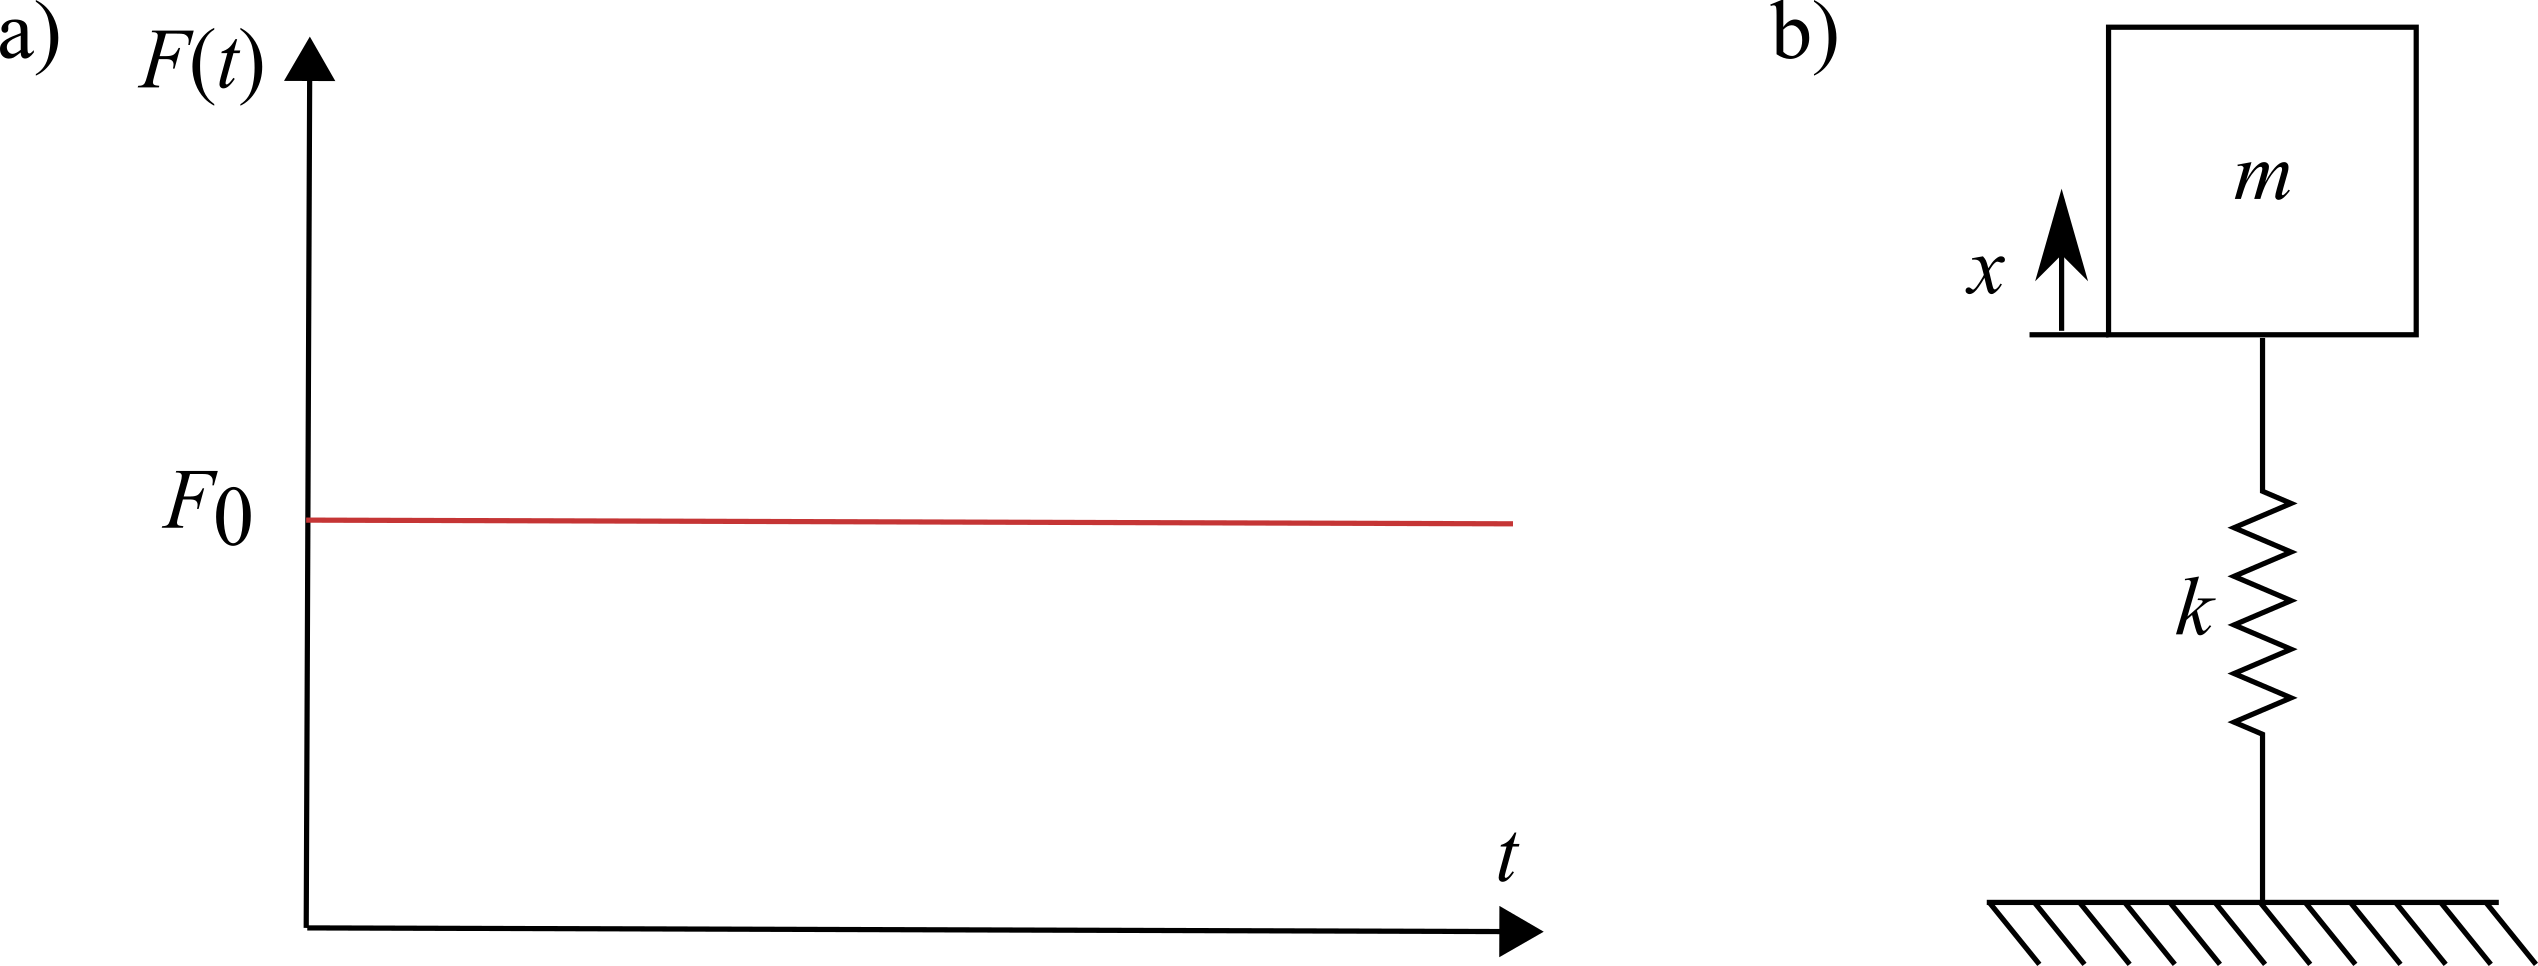
\includegraphics{../figures/structural_step_function_example.png}
		\caption{(a) Step function force; (b) undamped SDOF system.}
		\label{fig:step_force}
	\end{figure}

\vspace{1ex}
	
\noindent $Solution$:
	
\vspace{1ex}
	
The system is undamped, therefore we can use the Duhamel's integral in Eq. (\ref{Eq_Duhamel_undamped}) to find $x(t)$:

\begin{equation} 
x(t) = \frac{1}{m \omega_n} \int_{0}^{t} F_0 sin(\omega_n (t - \tau)) d\tau 
\end{equation}

Considering that $F_0$ is constant:

\begin{equation}
x(t) = \frac{F_0}{m \omega_n} \left [\frac{cos(\omega_n (t - \tau))}{\omega_n} \right ]_{0}^t = \frac{F_0}{m \omega_n^2} [1 - cos(\omega_n t)]
\end{equation}

Reminding that $\omega_n^2 = k/m$, $x(t)$ becomes:

\begin{equation}
x(t) = \frac{F_0}{k} [1 - cos(\omega_n t)]
\end{equation}

where $\frac{F_0}{k}$ is the displacement that the system would undergo if the force $F_0$ was applied statically.

In the case of underdamped SDOF system, the response becomes:

\begin{equation} 
x(t) = \frac{F_0}{k} \left [1 - e^{-\zeta \omega_n t} \left (cos(\omega_d t) + \frac{\zeta}{\sqrt{1 - \zeta^2}} sin(\omega_d t)\right) \right]
\end{equation}

\end{example}

%%%%%%%%%%%%%%%%%%%%%%%%%%%%%%%%%%%%%%%%%%%%%%%%%%%%%%%%%%%%%%%%%%%%%%%%%%%%%%%%%%%%%%%%%%%%%%%%%%%%%%%%%%%%%%%%%%%%%%%%%%%%%%%%%%%%%%%%%%%%%%%%

\subsection{Two-story frame}

The concepts discussed in Sec. 1 can be extended to the 2-story frame represented in Fig. \ref{fig:two_story_frame}. In fact, a 2-story frame can be modeled as a 2-DOF system under the following assumptions:

\begin{itemize}
	\item shear building: flexible columns ($EI \neq 0$), beam infinitely rigid ($EI_b$ = $\infty$), axial deformations of beams and columns negligible ($EA$ = 0);
	\item lumped mass system: floor-mass concentrated at the floor level.
\end{itemize}

\noindent Under such assumptions and free vibrations, we expect that the building moves following the deformed shape reported in Fig. \ref{fig:two_story_frame} (dotted line). Let's call the degrees of freedom of the frame $x_1(t)$ and $x_2(t)$. 

\begin{figure}[H]
	\centering
	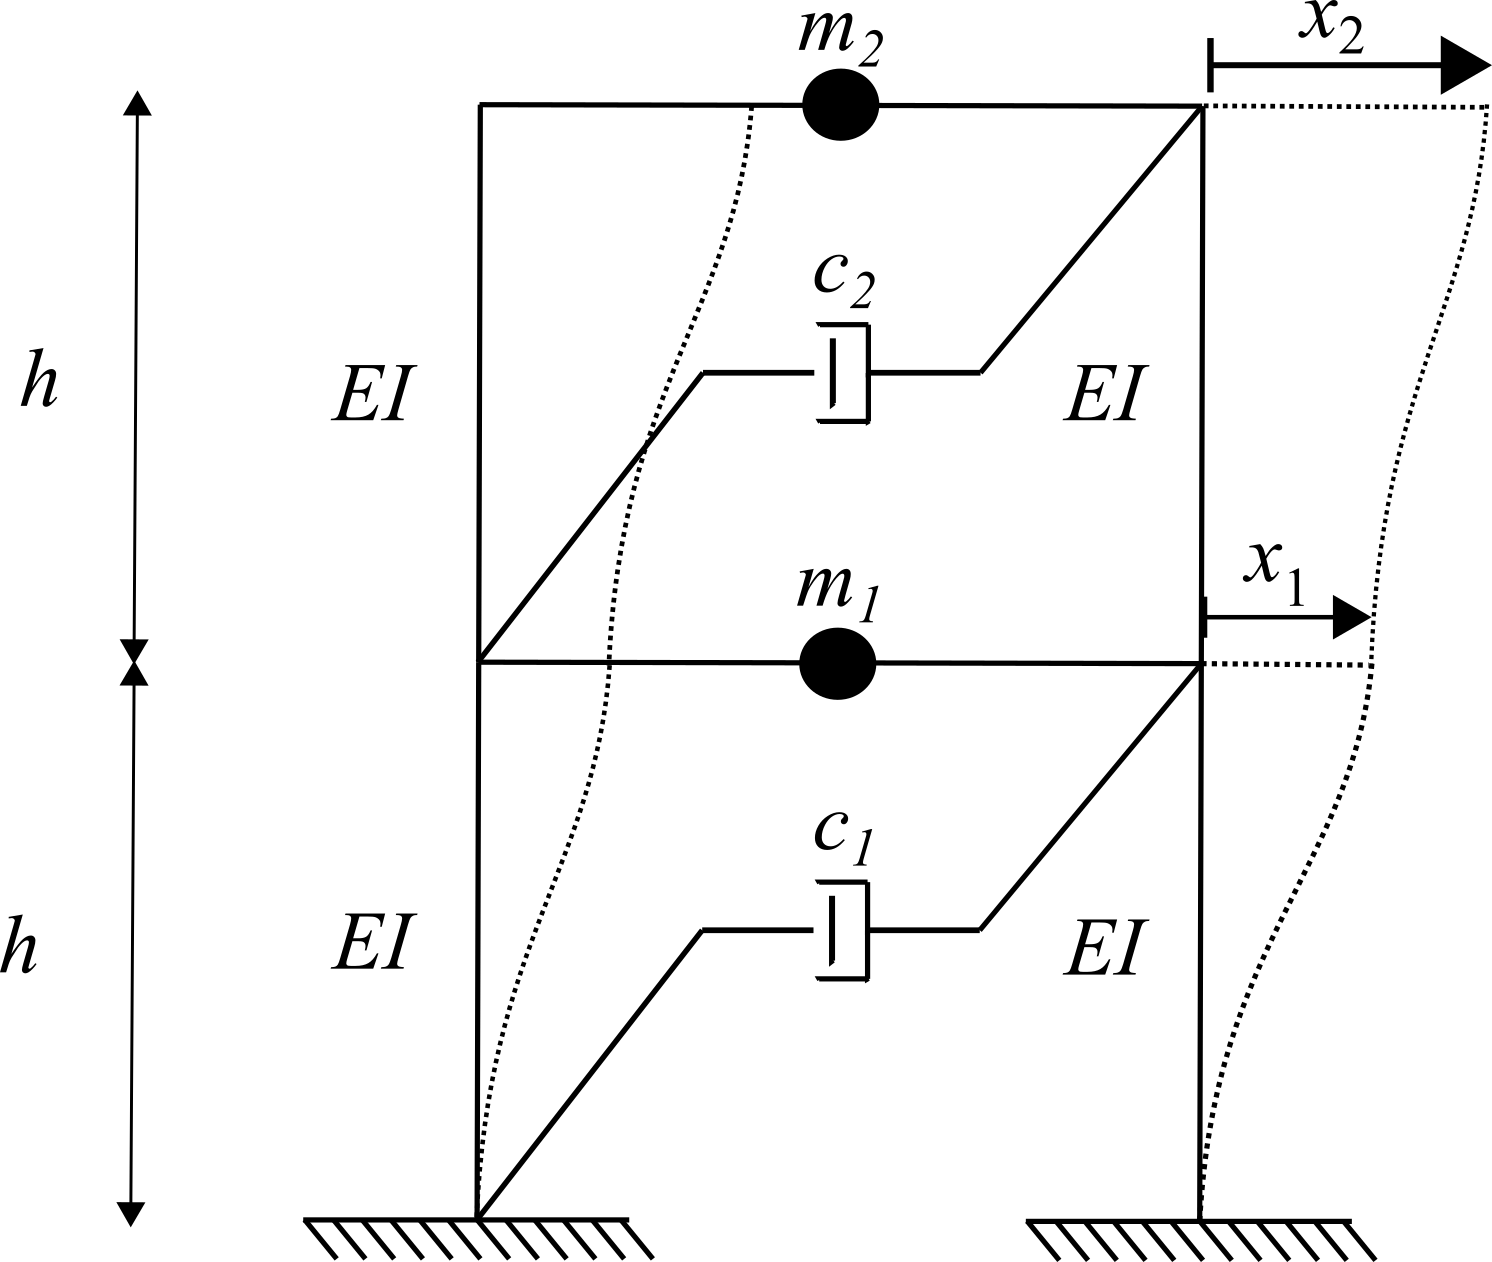
\includegraphics{../figures/two_story_frame.png}
	\caption{2-story frame with lumped masses.}
	\label{fig:two_story_frame}
\end{figure}


The forces acting on the 2-DOF system are reported in Fig. \ref{fig:twodof}. It follows that the equation of motion of the two masses are:

\begin{eqnarray}
m_1\ddot{x}_1 +k_1 x_1 + k_2 (x_2 - x_1) + c_1 \dot{x}_1\ + c_2 (\dot{x}_2 - \dot{x}_1) = 0\\
m_2\ddot{x}_2 - k_2 (x_2 - x_1) - c_2 (\dot{x}_2 - \dot{x}_1) = 0 \nonumber
\end{eqnarray}

\begin{figure}[h]
	\centering
	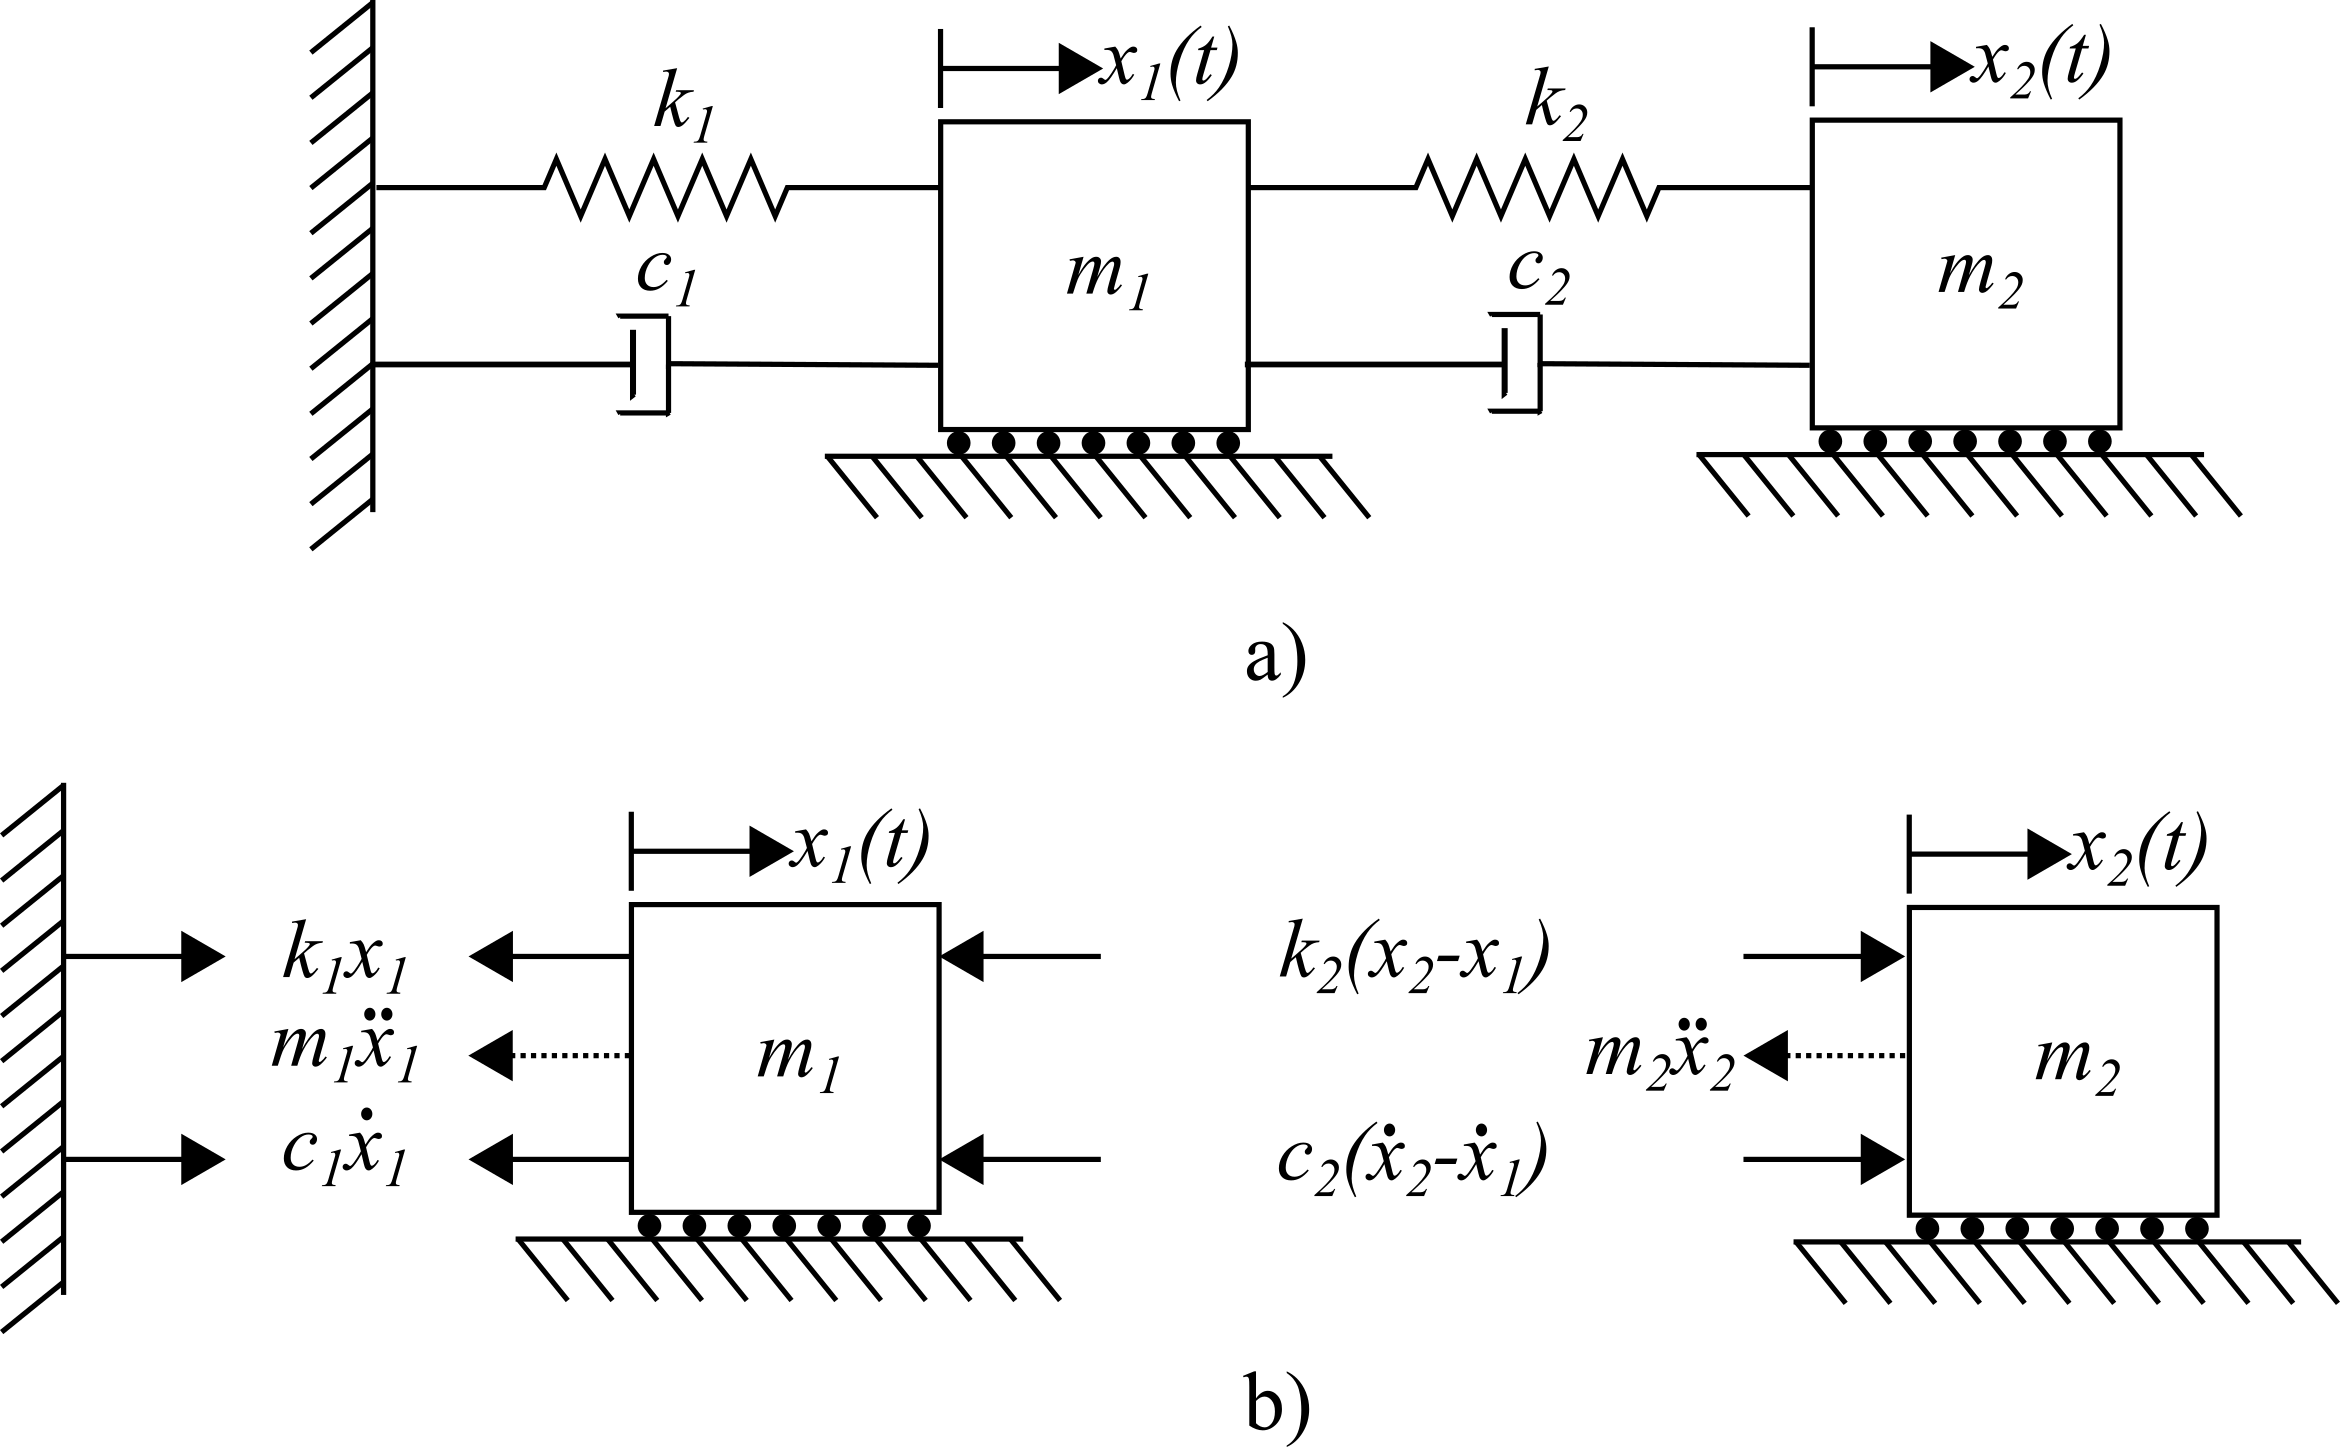
\includegraphics{../figures/2DOF_system.png}
	\caption{(a) 2-DOF system used to model the 2-story frame; (b) free body diagram of the two masses.}
	\label{fig:twodof}
\end{figure}



In matrix notation, these two equations become:

\begin{eqnarray} \label{EOM2DOF}
\begin{bmatrix} m_1 & 0  \\  0 & m_2 \end{bmatrix}\begin{bmatrix} \ddot{x_1} \\  \ddot{x_2} \end{bmatrix} + \begin{bmatrix} k_1+k_2 & -k_2  \\  -k_2 & k_2 \end{bmatrix}\begin{bmatrix} x_1 \\  x_2 \end{bmatrix} + \begin{bmatrix} c_1 + c_2 & -c_2  \\  -c_2 & c_2 \end{bmatrix}\begin{bmatrix} \dot{x}_1 \\  \dot{x}_2 \end{bmatrix} = \begin{bmatrix} 0 \\  0 \end{bmatrix}
\end{eqnarray}

\noindent where we can define the mass matrix $M$ as:
		
\begin{eqnarray}
M=  \begin{bmatrix} m_1 & 0  \\  0 & m_2 \end{bmatrix}  
\end{eqnarray}

\noindent the stiffness matrix $K$ as:
\begin{eqnarray}
K=  \begin{bmatrix} k_1+k_2 & -k_2  \\  -k_2 & k_2 \end{bmatrix}
\end{eqnarray}		
		
\noindent and the damping matrix $C$ as:
\begin{eqnarray}
C=  \begin{bmatrix} c_1+c_2 & -c_2  \\  -c_2 & c_2 \end{bmatrix}
\end{eqnarray}
		
		
While mass and damping of a frame are usually given, the stiffness values $k_1$ and $k_2$ need to be calculated as a function of the columns properties ($EI$) and geometry ($h$). As demonstrated in Sec. 1, the stiffness of a column with clamped ends can be determined as:

\begin{equation}
k_c = \frac{12EI}{h^3}
\end{equation}

The lateral stiffness of each floor can be computed as the sum of the stiffness of the columns at that floor:

\begin{equation}
k = \sum_{columns}^{} k_c = \sum_{2}^{} \frac{12EI} {h^3}
\end{equation}
		
Therefore, for the frame in Fig. \ref{fig:two_story_frame}, the stiffness values are:
		
\begin{equation}
k_1 = k_2 = \frac{24EI}{h^3}
\end{equation}
		
The solution of the EOM in Eq.(\ref{EOM2DOF}) was derived in Chapter 5 and can be summarized as:

\begin{equation}
\begin{bmatrix} x_1(t) \\  x_2(t) \end{bmatrix} =  \begin{bmatrix} \mathbf{u}_1 & \mathbf{u}_2 \end{bmatrix}
\begin{bmatrix} A_1 \sin (\omega_1 t + \phi_1 )\\ A_2 \sin (\omega_2 t + \phi_2 )\end{bmatrix}, \hspace{1cm} \omega_1 \text{ or } \omega_2 \neq 0
\end{equation}

\noindent where $\mathbf{u}_1$ and  $\mathbf{u}_2$ are eigenvectors (or mode shapes), $\omega_1$ and $\omega_2$ are the natural frequency of vibration, 
$\phi_1$, $\phi_2$, $A_1$, and $A_2$ are constants that can be found based on the initial conditions (see Chapter 5 for more details).

\vspace{4ex}

%%%%%%%%%%%%%%%%%%%%%%%%%%%%%%%%%%%%%%%%%%%%%%%%%%%%%%%%%%%%%%%%%%%%%%%%%%%%%%%%%%%%%%%%%%%%%%%
		
\begin{example}

Consider the frame in Fig. \ref{fig:two_story_frame_ex}. Determine natural frequency of vibration and mode shapes of the system.

\begin{figure}[H]
	\centering
	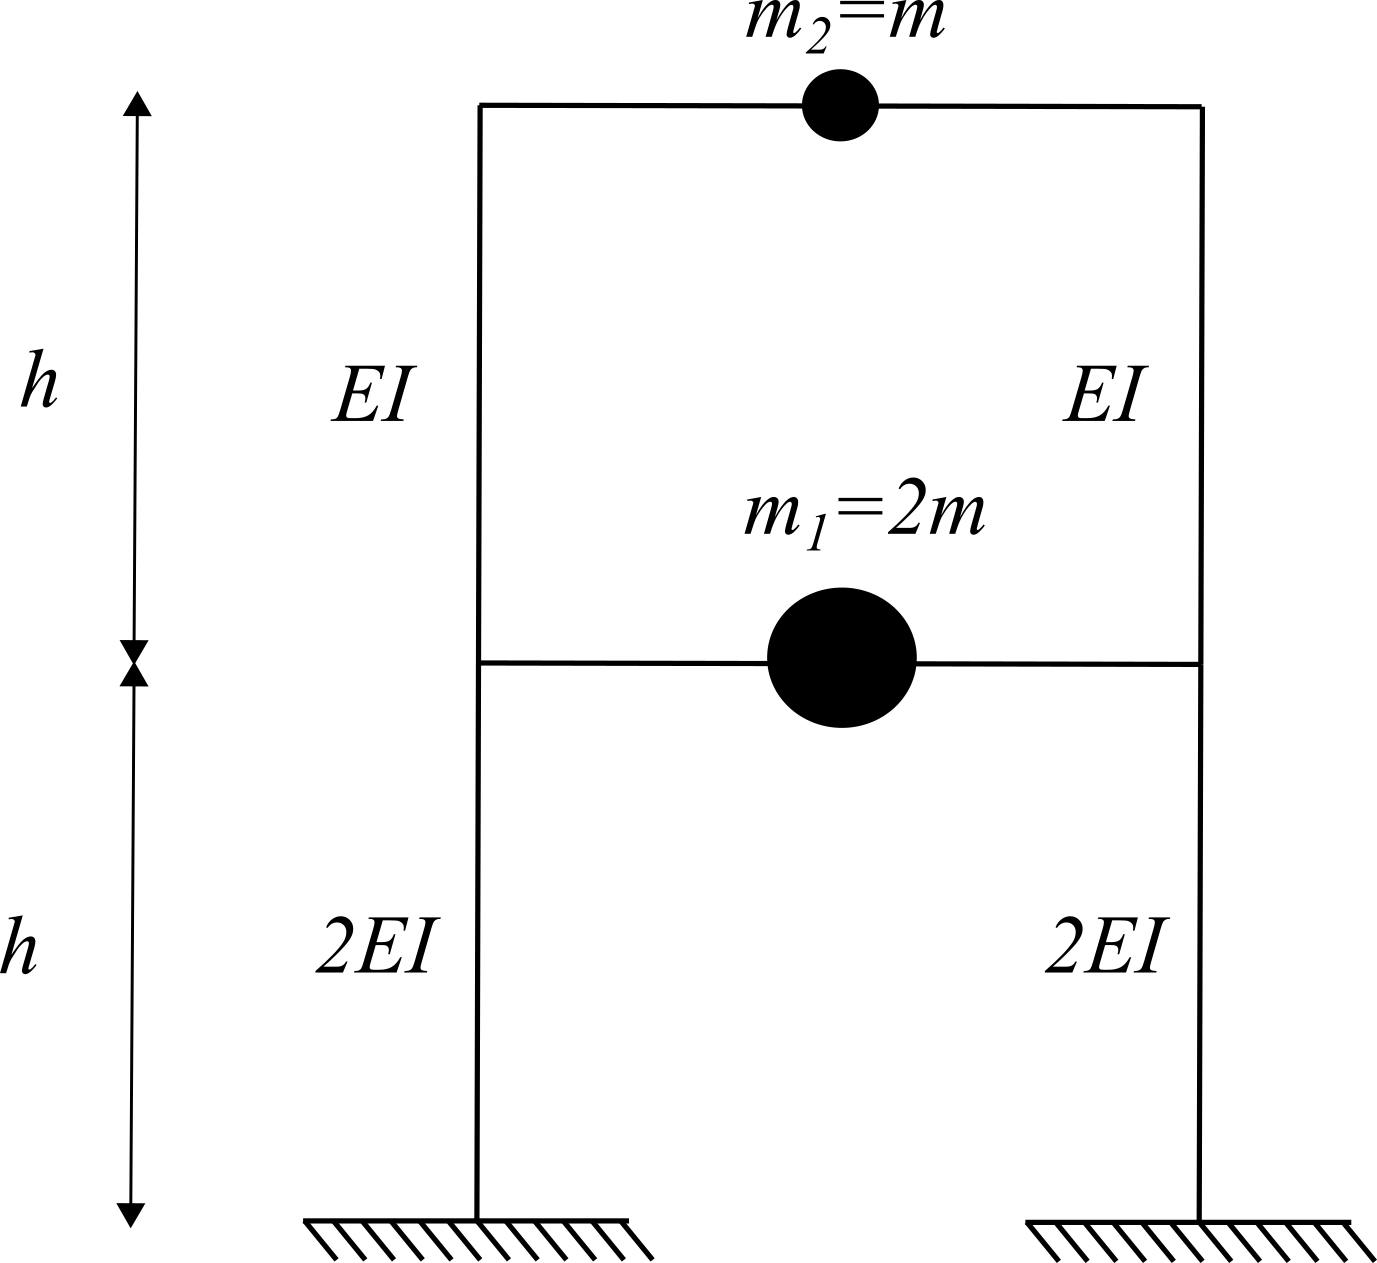
\includegraphics{../figures/two_story_frame_example.png}
	\caption{Example of a 2-story frame with floors with different dynamic properties.}
	\label{fig:two_story_frame_ex}
\end{figure}




\noindent $Solution$:

\vspace{1ex}
	
Assumption: the frame can be modeled as a shear building with mass lumped at the floor levels. The lateral stiffness at the first floor is:

\begin{equation}
k_1 = 2 \frac{12(2EI)}{h^3} = \frac{48EI}{h^3}
\end{equation}

\noindent The lateral stiffness at the second floor is:
\begin{equation}
k_2 = 2 \frac{12(EI)}{h^3} = \frac{24EI}{h^3}
\end{equation}

\noindent Therefore, the stiffness matrix can be written as:

\begin{eqnarray}
K= \begin{bmatrix} \frac{48EI}{h^3} + \frac{24EI}{h^3} & -\frac{24EI}{h^3}  \\  -\frac{24EI}{h^3} & \frac{24EI}{h^3} \end{bmatrix} = \frac{24EI}{h^3} \begin{bmatrix} 3 & -1  \\  -1 & 1 \end{bmatrix}
\end{eqnarray}		


The EOM of the system is:

\begin{eqnarray} 
\begin{bmatrix} 2m & 0  \\  0 & m \end{bmatrix}\begin{bmatrix} \ddot{x_1} \\  \ddot{x_2} \end{bmatrix} + \frac{24EI}{h^3} \begin{bmatrix} 3 & -1  \\  -1 & 1 \end{bmatrix}\begin{bmatrix} x_1 \\  x_2 \end{bmatrix}  = \begin{bmatrix} p_1 \\  p_2 \end{bmatrix}
\end{eqnarray}

In order to determine the natural frequency of vibration and the mode shapes of the system, we need to solve the characteristic equation:

\begin{equation}
\det(-\omega^2 M  + K) = 0
\end{equation}

\noindent leading to:

\begin{equation}
2m^2 \omega^4 + 5 k m \omega^2 + 2 k = 0
\end{equation}

\noindent This equation has two solutions:

\begin{eqnarray}
\omega_1^2 = \frac{k}{2 m}\\
\omega_2^2 = \frac{2 k}{m}
\end{eqnarray}

\noindent Therefore, the two natural frequencies of vibration of the system are:

\begin{eqnarray}
\omega_1 = \sqrt{\frac{k}{2 m}}\\
\omega_2 = \sqrt{\frac{2 k}{m}}
\end{eqnarray}

\noindent where $k = \frac{24EI}{h^3}$. The mode shapes of the frame can be found by solving the following equation:

\begin{equation}
(-\omega_1^2 M  + K)\mathbf{u}_1 =0
\end{equation}

\noindent Replacing mass and stiffness matrix the equation becomes:

\begin{equation}
\bigg(-\frac{k}{2 m}\begin{bmatrix}  2m & 0 \\   0  & m \end{bmatrix} + k \begin{bmatrix} 3 & -1 \\    -1  & 1 \end{bmatrix}\bigg)\begin{bmatrix} u_{11}\\ u_{21}\end{bmatrix} = \begin{bmatrix} 0\\ 0\end{bmatrix}
\end{equation}

\noindent simplified to

\begin{equation}
\begin{bmatrix} 2k & -k \\    -k  & \frac{k}{2} \end{bmatrix} 
\begin{bmatrix} u_{11}\\ u_{21}\end{bmatrix}=\begin{bmatrix} 0\\ 0\end{bmatrix}
\end{equation}

\noindent leading to two equations:

\begin{equation}
2 k u_{11} -k u_{21}=0 \text{, and } -k u_{11} + \frac{k}{2} u_{21}=0
\end{equation}

\noindent It follows that:
\begin{equation}
2 u_{11}= u_{21}  \text{, and } u_{11} = \frac{1}{2}u_{21}
\end{equation}

\noindent To obtain a numerical value, we arbitrarily assign a value to one of the elements. Here, let $u_{21}=1$ so let $u_{11}=1/2$. Therefore, 
\begin{equation}
\textbf{u}_1 = \begin{bmatrix} \frac{1}{2}\\ 1\end{bmatrix}
\end{equation}

\noindent Similarly, $\mathbf{u}_2$ can be obtained by solving the following equation:

\begin{equation}
(-\omega_2^2 M  + K)\mathbf{u}_2 =0
\end{equation}

\noindent leading to:

\begin{equation}
	\textbf{u}_2 = \begin{bmatrix} -1\\ 1\end{bmatrix}
\end{equation}

\noindent Fig. \ref{fig:modeshapes} represents the two mode shapes of the building. 

\vspace{4ex}

\begin{figure}[H]
	\centering
	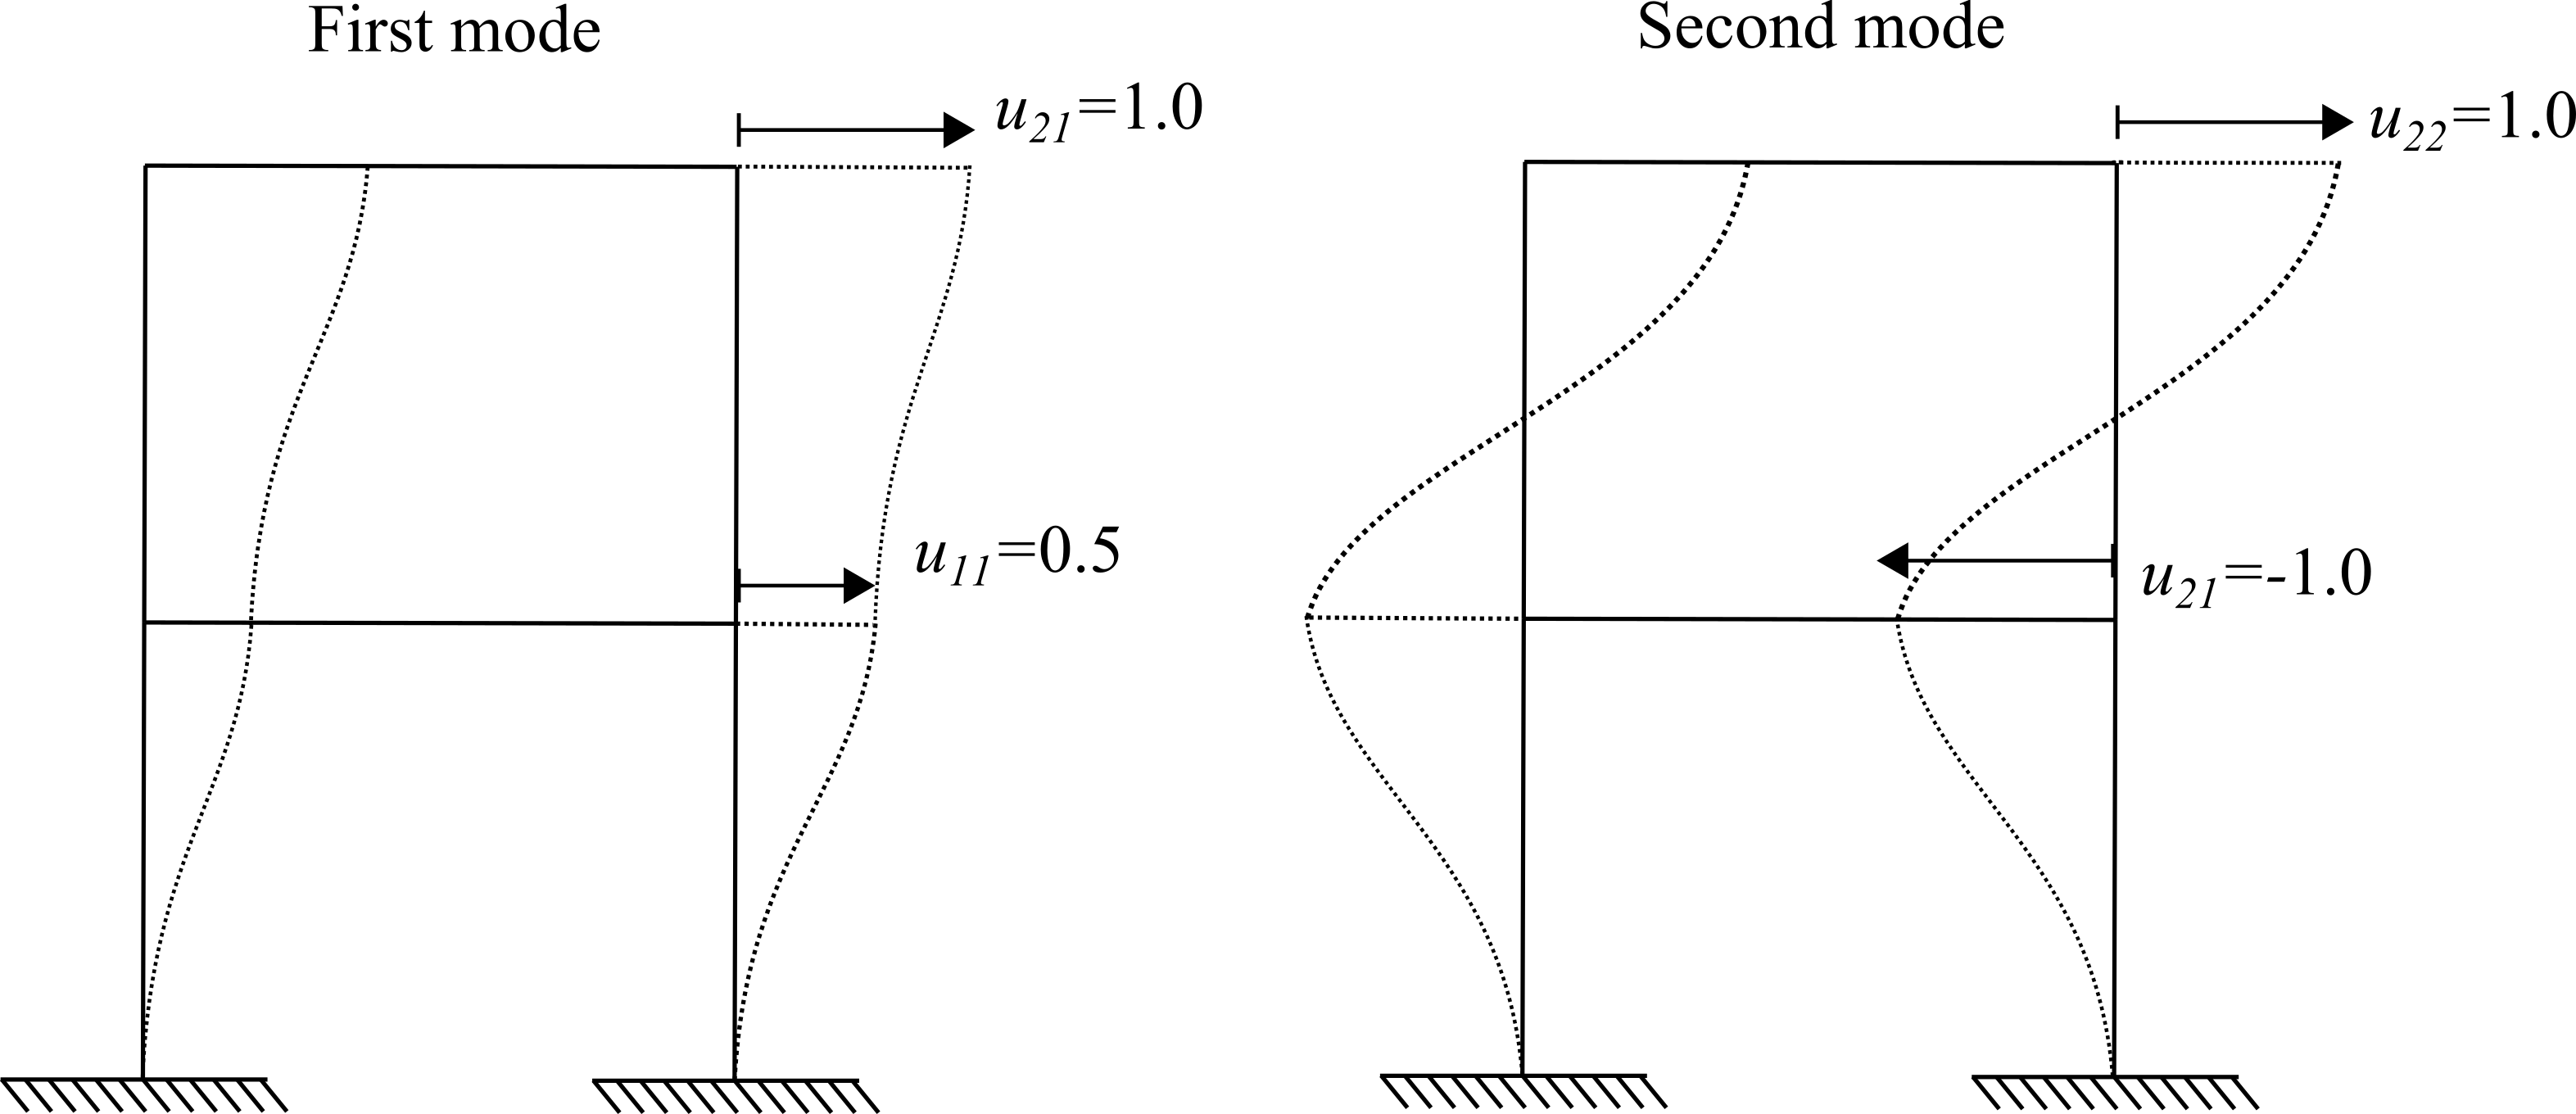
\includegraphics{../figures/two_story_frame_example_mode_shapes.png}
	\caption{Mode shapes of the 2-story frame.}
	\label{fig:modeshapes}
\end{figure}

\pagebreak


The temporal response of the system is given by:

\begin{equation}
\begin{bmatrix} x_1(t) \\  x_2(t) \end{bmatrix} =  \begin{bmatrix} \mathbf{u}_1 & \mathbf{u}_2 \end{bmatrix}
\begin{bmatrix} A_1 \sin (\omega_1 t + \phi_1 )\\ A_2 \sin (\omega_2 t + \phi_2 )\end{bmatrix}, \hspace{1cm} \omega_1 \text{ or } \omega_2 \neq 0
\end{equation}

where $\mathbf{u} = [\mathbf{u}_1, \mathbf{u}_2]$ is the time invariant part of the equation. 


\end{example}
		

		
		
		
\end{document}













